\documentclass[12pt,english]{scrartcl}

\usepackage{amsmath,amssymb}
%\usepackage[amssymb]{SIunits}
\usepackage{babel}
\usepackage[latin1]{inputenc}
\usepackage{graphicx}
\usepackage{color}
\usepackage{url}


\begin{document}

\begin{center}
\textbf{\begin{LARGE}KOGW-PM-KNP:\\ \vspace{3mm} Tutorial 10 - Spacing effects in learning
\end{LARGE}}
\end{center}

This tutorial deals with a strategies to optimize retention of learned material. The paper by Cepeda et al., (2008) conducts a large scale internet study and argue - based on their results - that many educational practices are highly inefficient. Please read the paper carefully. Answer the following questions which should help you to evaluate their findings. Please work in pairs. 
%  
% \begin{figure}[htbp]
% \begin{center}
% 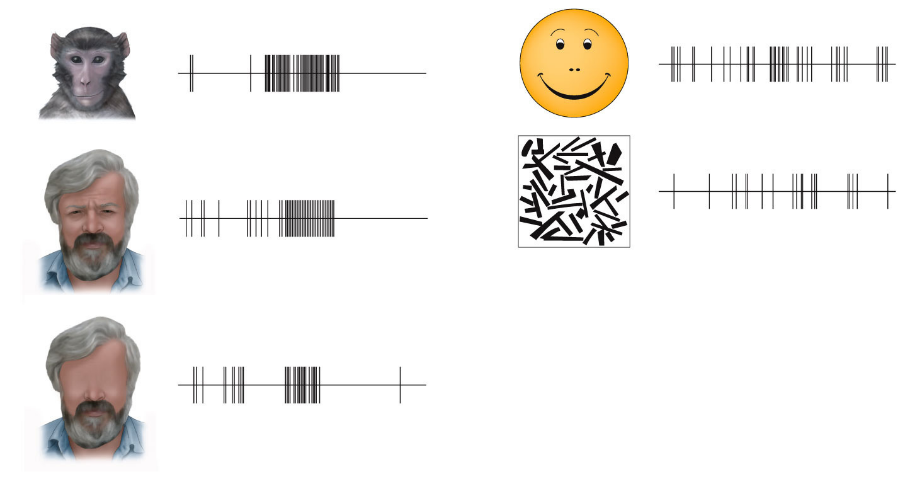
\includegraphics[width = 0.8\textwidth]{IT_cell.png}
% \end{center}
% \caption{
% \label{fig:IT_cell}}
% \end{figure}

\begin{enumerate}
 \item What was the research question addressed by the authors?

 \color{blue}
 \begin{itemize}
 \item How does the gap between multiple exposure to to-be-learned material affect subsequent forgetting?
 \end{itemize}
  \color{black}

 \item Explain the typical design and result pattern of experiments on spacing effects or effects of distributed practice.

 \color{blue}
 \begin{itemize}
 \item multiple periods of study devoted to the same material
 \item periods separated by variable time gaps
 \item final memory test after an additional retention interval measured from the final study episode
 \item[]
 \item worst performance in no gap condition, best performance for intermediate gap duration  
 \end{itemize}
  \color{black}

 \item What was reported in the study by Bahrick et al., 1993? What potential confound do the present authors identify in their study?
 
\color{blue}
 \begin{itemize}
 \item foreign language vocabulary of 4 subjects
 \item retention inverals of 1, 2, 3, 4 years
 \item gap between study periods of 14, 28, 56 days
 \item[]
 \item results: monotonically increasing performance across the tested study intervals 
 \item confound: subjects trained to fixed criterion in each study session - longer gaps might have required more relearning trials
 \end{itemize}
  \color{black}

 \item What was the goal of the present study?

 \color{blue}
 \begin{itemize}
 \item examine joint effects of gap and retention interval (RI) more systematically and over longer time intervals than has been previously done
 \item held constant the number of restudy trials in the second study session - separate effect of gap and amount of time provided for restudy
 \item greater range of gap/RI ratios - assess generality of non-monotonic relationship between retention performance and gap
\end{itemize}
  \color{black}


 \item Describe the procedure and the results of the preliminary study. Was that a within- or a between-subjects design, why?

 \color{blue}
 \begin{itemize}
 \item 150 subjects learned random associations between facts or objects' names
 \item gaps between 10min and 6 months 
 \item final memory test 6 months after second learning session
 \item recall for facts and names was best for a 1-month gap (1/6month)
 \item between subjects design- otherwise gap sizes confounded
\end{itemize}
  \color{black}


 \item Describe the design and procedure of the main study.

 \color{blue}
 \begin{itemize}
 \item 1.354 subjects learned random associations between facts or objects' names
 \item gaps: 0, 1, 2, 4, 7, 14, 21, 35, 70, 105
 \item RI: 7d, 35d, 70d, 350d (1 week, 1 month, 2 months, 1 year)
 \item gap/RI ratios of 0.1, 0.2, 0.3
 \item first learning: 32 facts learned to criterion of one perfect recall (European nation that consumes most spicy Mexican food? - Norway)
 \item second learning: tested twice on each fact, correct answer was shown after each response
 \item final test: recall without FB, recognition: pick the correct answer from 5 options
 \item[!] questions answered correctly on the very first test were assumed to be known by the subject and excluded from all subsequent analysis for that person 
\end{itemize}
  \color{black}

\item The present results show that the timing of learning sessions can have powerful effects on retention when study time is equated. What is the major educational implication of this  result? Will that have an effect on your own study behavior?
 \color{blue}
 \begin{itemize}
 \item spacing depends on how long you want to retain something
 \item long-term retention: delayed review of at least several months 
\end{itemize}
  \color{black}


 \item Describe the results of the main study.

 \color{blue}
 \begin{itemize}
 \item inverted U-shape for retention performance as a function of gap size
 \item optimal gap as compared to zero-day gap provided a 64\% increase in final recall and 26\% increase in final recognition
 \item optimal gaps for RI of 7, 35,70, 350 days were 1, 11, 21, 21 days $\Rightarrow$ .14, .31,.3,.06
 \item agreement with lab benchmark
 \item optimal gaps departed form fixed proportion of RI

\end{itemize}
  \color{black}


\item List potential objections against Internet-based testing. Do you think the authors satisfactorily address the concerns?
 \color{blue}
 \begin{itemize}
 \item Internet subjects have more distractions than subjects tested in the lab (more noise reduced effect size)
 \item possibility of cheating (suprisingly good performance > 85\% 2.6 vs 2.1\% Internet vs lab)
\end{itemize}
  \color{black}
 
\end{enumerate}

\end{document}
